\documentclass{article}

\def\pdfpsfrag{no}
\def\reusepsfragpdf{yes or no}
\def\foiltex{no}
\def\algfontmode{no}
\input{../../FrequentlyUsed/latex/mydefs}

\usepackage{fullpage}
\usepackage{tikz}
\usetikzlibrary{decorations.pathreplacing}

\title{Dynamics systems in Physics}
\author{Sunghee Yun - Beth's Daddy \& Liam, Lucy, Adrian \& Lillian's Uncle}

\begin{document}
\maketitle
\tableofcontents

\newpage

\section{Introduction}

It was when I helped Beth, the most lovely daughter in the world, prep her physics final exam
where we solved the dynamics problem shown in \figurename~\ref{fig:high-school-physics-problem}
that I felt this urge to want to see how things with masses actually move in the field of gravity and springs and all that in the real world
(or rather in a virtual world \verb+*^^*+).

To solve the exercise problem was not smooth all along, but after being reminded of what I studied in my high school and college,
we finally got it. Then Beth threw another question of at what point the speed of the box is maximized?
We first thought that it is when the box touches the spring, but soon we realized that that is not correct.
We figured to figure it out, we have to find a point where the total potential energy,
\ie, by the gravity and the spring, is minimized
because the kinetic energy is maximized at that point
due to the law of conservation of energy.

Then I don't know why (like in most of such cases),
but I really had to start developing Python software
simulating the motions of these objects. :)

So here I am, and I've developed the package called {\tt science}
(yes, the name is too generic, I may come up with a different name soon).
With {\tt science},
one can specify the point masses with their initial locations and velocities,
springs with spring constants and natural lengths,
frictional forces with the coefficient of friction,
\etc\
to simulate the motions.

In this document,
I will write the laws, formula, equations, theories, and related proof
with some examples generated by {\tt science}.

\begin{figure}
\begin{center}
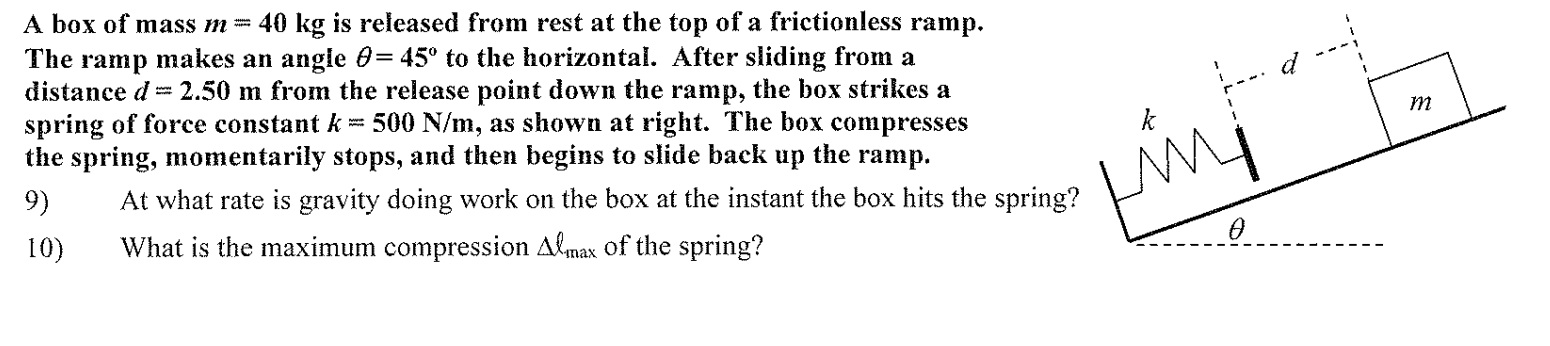
\includegraphics[trim = 10 40 20 05, clip, width=.9\textwidth]{figures/physics-problem}
\end{center}
\caption{A physics problem that I solved with Beth to prep the final}
\label{fig:high-school-physics-problem}
\end{figure}

\section{Resource}

\begin{itemize}
\item
	This document can be found \href{https://github.com/sungheeyun/science/blob/main/docs/dynamics-equations.pdf}{here}.
\item
	GitHub repository - {\tt \href{https://github.com/sungheeyun/science}{https://github.com/sungheeyun/science}}

\item
	The main Python script - {\tt \href{https://github.com/sungheeyun/science/blob/main/bin/simulation-dynamics.py}{simulation-dynamics.py}}

\item
	Some example YAML input files can be found \href{https://github.com/sungheeyun/science/tree/main/data/input}{here}.
\end{itemize}


\section{Force equations}

\subsection{Ideal springs}

Suppose (simple) rules for springs hold. That is when a spring with $k\in\ppreals$ as the spring constant and $l\in\ppreals$ as the natural length
and two point masses $m_1\in\ppreals$ and $m_2\in\ppreals$, which are located at
$x_1\in\reals^3$
and
$x_2\in\reals^3$
as show in \figurename~\ref{fig:spring}.
The force exerted on $m_1$ is
\begin{equation}
\label{eq:force:spring}
	F_s(x_1;k,l,x_2) = -k (\|x_1-x_2\| - l) v_{2,1}
	= -k
	\left(
	\frac{\|x_1-x_2\| - l}{\|x_1-x_2\|}
	\right)
	(x_1-x_2)
\end{equation}
where $v_{2,1}\in\reals^3$ is a unit-length vector pointing to the direction of $x_1-x_2$,
\ie,
\[
	v_{2,1} =
%	\left(
	\frac{1}{\|x_1-x_2\|}
%	\right)
	(x_1-x_2).
\]
Here $\|x\|$ is the $2$-norm or the size of a vector $x\in\reals^3$ defined by
\[
	\|x\| = \sqrt{x_1^2+x_2^2+x_3^2}.
\]

The force exerted on $m_2$ $F_s(x_2;k,l,x_1)$ be can obtained using

\begin{figure}
\begin{center}
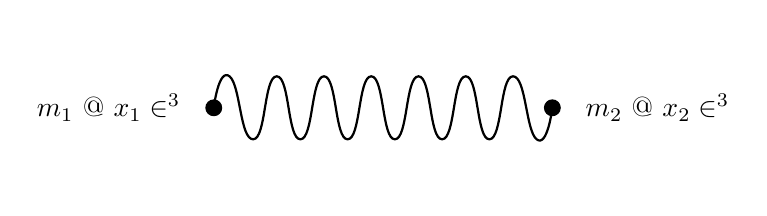
\begin{tikzpicture}[scale=1]
\def\coils{6} % Number of coils
\def\radius{0.4} % Radius of coils
\def\length{5} % Total length of spring
\def\startx{-2} % Starting x coordinate
\def\starty{0} % Starting y coordinate
\def\slope{2} % Height increase over length

%    \draw[very thin, dashed] (-3.5, -1) rectangle (3.8, 1); % Rectangle boundary
	\node[inner sep=0pt, outer sep=0pt] (left) at (-3.5, 0) {};
    \node[inner sep=0pt, outer sep=0pt] (right) at (3.8, 0) {};
    \node[inner sep=0pt, outer sep=0pt] (top) at (0, 1) {};
    \node[inner sep=0pt, outer sep=0pt] (bottom) at (0, -1) {};
    % Draw balls

	\def\ballo{(-2, 0)}
    \def\ballt{(2.3, 0)}

    % Draw balls
    \draw[fill=black] \ballo circle (0.1); % Ball 1
    \draw[fill=black] \ballt circle (0.1); % Ball 2

	\node[left=.3cm] at (-2, 0) {$m_1$ @ $x_1\in\reals^3$};
    \node[right=.3cm] at (2.3, 0) {$m_2$ @ $x_2\in\reals^3$};

\draw[thick] plot[smooth, tension=1]
  coordinates {
    (\startx+0.0,\starty)
    (\startx+0.2,\starty+\radius)
    (\startx+0.5,\starty-\radius)
    (\startx+0.8,\starty+\radius)
    (\startx+1.1,\starty-\radius)
    (\startx+1.4,\starty+\radius)
    (\startx+1.7,\starty-\radius)
    (\startx+2.0,\starty+\radius)
    (\startx+2.3,\starty-\radius)
    (\startx+2.6,\starty+\radius)
    (\startx+2.9,\starty-\radius)
    (\startx+3.2,\starty+\radius)
    (\startx+3.5,\starty-\radius)
    (\startx+3.8,\starty+\radius)
    (\startx+4.1,\starty-\radius)
    (\startx+4.3,\starty)
  };
\end{tikzpicture}
\end{center}
\caption{A spring connecting two point masses}
\label{fig:spring}
\end{figure}

\subsection{Gravity-like forces}

In a real world we live, we feel the gravity dragging us downward.
But since we can assume anything here! :)
let us assume that there exists gravity-like force
in a sense that given an acceleration vector $a\in\reals^3$,
the force exerted on a point mass $m\in\ppreals$ located at $x\in\reals^3$
is
\begin{equation}
\label{eq:force:gravity-like}
F_g(m;a) = ma
	\in\reals^3
\end{equation}
\ie,
the magnitude of the force is proportional to $m$ (and the magnitude of the acceleration),
the direction is the same as that of the acceleration.
It does \emph{not} depend on the location.

A typical example, of course, is \emph{the} gravity where
\[
	a = (0,0,-g)
	\in\reals^3
\]
with $g = 9.8 m/s^2$.

\subsection{Frictional forces}
\label{subsection:frictional-forces}

We model frictional forces exerted on bodies (not point mass)
using the coefficient of friction $c\in\ppreals$ where the force is modeled by

\begin{equation}
\label{eq:force:frictional}
F_f(v) = -c v
	\in\reals^3
\end{equation}
where $v\in\reals^3$ is the velocity along the surface.

\section{Energies}

\subsection{Kinetic energy of a mass}

The kinetic energy of a mass $m$ with velocity $v\in\reals^3$
is defined by
\begin{equation}
\label{eq:energy:kinetic}
	E_\mathrm{k}(m) = \frac{m}{2} \|v\|^2
\end{equation}

\subsection{Potential energy}

Note that the role of the potential energies in dynamics
is played in a way that the difference of them at two location,
hence adding a constant to any potential energy
makes no difference.

\subsubsection{Potential energy by a gravity-like force}

The potential energy of a mass $m$ by a gravity-like force with acceleration $a\in\reals^3$
is defined by
\begin{equation}
\label{eq:energy:potential:gravity-like}
E_\mathrm{p,g}(m,x;a)
=  - m x\cdot a
= - m x^Ta
\end{equation}
where $a^Tb = a\cdot b$ for two vectors $a$ and $b$
is the inner product defined by
\[
	(a_1,a_2,a_3) \cdot (b_1,b_2,b_3) = a_1b_1 + a_2b_2 + a_3b_3.
\]
For example, the potential energy by gravity is
\[
	E_\mathrm{p,g}(m,x;g)
	= -(0,0,-g) \cdot (x_1,x_2,x_3)
	=  mgx_3
\]

\subsubsection{Potential energy by a spring}

The potential energy of a mass $m$ by a gravity-like force with acceleration $a\in\reals^3$
is defined by
\begin{equation}
\label{eq:energy:potential:spring}
E_\mathrm{p,s}(x_1,x_2;k,l)
= \frac{k}{2} (\|x_1-x_2\|-l)^2
\end{equation}


\subsection{The law of conservation of energy}

In a system with masses, springs, and gravity-like forces with no frictional forces,
the sum of the kinetic energies of all the masses
and that of the potential energies of all the gravity-like forces and springs
is conserved
unless, for example, external forces are exerted on the system,
two point masses merge into one,
or some non-elastic crashes happen.

\paragraph{Proof}
\label{paragraph:proof}

Suppose that the location of a point mass $m$ is $x(t)\in\reals^3$
and the force exerted on $m$ is $F(t)\in\reals^3$ where $t$ refers to the time.
These notations explicitly show that both quantities are functions of time $t$.
The Newton's second law, $F(t) = m a(t)$ where $a(t) = \frac{d}{dt^2}x(t)$ is the acceleration of $m$,
implies
\begin{eqnarray}
\nonumber
\lefteqn{
\int_{t_1}^{t_2} (-F(t)) \cdot d x
 = - \int_{t_1}^{t_2} m a(t) \cdot d x
 = - \int_{t_1}^{t_2} m \left( \frac{dv(t)}{dt} \right) \cdot v(t) dt
}\\
 &=& - \int_{t_1}^{t_2} m {v(t)} \cdot dv(t)
= - \left(
 	\frac{m}{2}v(t_2)^2 - \frac{m}{2} v(t_1)^2
 \right)
=
\frac{m}{2} v(t_1)^2
- \frac{m}{2}v(t_2)^2
\label{eq:energy:conserve:1}
\end{eqnarray}
where we use the definition of velocity,
$v(t) = {dx(t)}/{dt}$.

Now we will show that $\int (-F(t)) dt $ is the same as (the difference of) the potential energies defined for
the gravity-like force and the spring respectively.
For the gravity-like force,
we have
\begin{equation}
\label{eq:potential-energy-gravity-like}
	\int_{t_1}^{t_2} (-F_g(m;a)(t))\cdot dx
=
	-m \int_{t_1}^{t_2} a\cdot dx
=
	-m (a\cdot x(t_2) - a\cdot x(t_1))
=
	E_\mathrm{p,g}(t_2)
	-
	E_\mathrm{p,g}(t_1).
\end{equation}
For the spring,
%we have
we re-parameterize the coordinates of $x_1$ using $r\geq0$, $-\pi/2\leq \phi \leq \pi/2$, $0\leq \theta < 2\pi$
\[
(x_{1,1}, x_{1,2}, x_{1,3}) = (x_{2,1} + r \cos\phi \cos\theta, x_{2,2} + r \cos\phi \sin\theta, x_{2,3} + r \sin\phi).
\]
Then we have
\begin{eqnarray*}
\|x_1 - x_2\|
&=&
\|
r( \cos\phi \cos\theta,  \cos\phi \sin\theta,  \sin\phi)
\|
=r
\\
d x_{1,1}
&=&
\cos\phi \cos\theta dr
-r\sin\phi \cos\theta d\phi
-r\cos\phi \sin\theta d\theta
\\
d x_{1,2}
&=&
\cos\phi \sin\theta dr
- r \sin\phi \sin\theta d\phi
+ r \cos\phi \cos\theta d\theta
\\
d x_{1,3}
&=&
\sin\phi dr
+ r \cos\phi d\phi
\end{eqnarray*}
hence
by (\ref{eq:force:spring})
\[
-F_s(x_1;k,l,x_2)\cdot dx_1
= k \left(\frac{r-l}{r}\right) rdr
= k (r-l) dr
= k (r-l) d(r-l),
\]
thus
\begin{equation}
\label{eq:potential-energy-gravity-like}
	\int_{t_1}^{t_2} (-F_s(x_1;k,l,x_2)(t))\cdot dx_1
=
	\frac{k}{2}(\|x_1(t_2)-x_2\|-l)^2
	-
	\frac{k}{2}(\|x_1(t_1)-x_2\|-l)^2
=
	E_\mathrm{p,s}(t_2)
	-
	E_\mathrm{p,s}(t_1)
\end{equation}
assuming only $m_1$ moves while $m_2$ does not.
We can generalize this argument where two masses $m_1$ and $m_2$
move simultaneously (though we will not show it here).

Therefore for both spring force and gravity-like force,
(\ref{eq:energy:conserve:1})
implies
\begin{equation}
\label{eq:energy-conserve-for-each-mass}
E_\mathrm{p}(t_2) - E_\mathrm{p}(t_1)
=
\frac{m}{2} v(t_1)^2
- \frac{m}{2}v(t_2)^2
\quad
\Leftrightarrow
\quad
\frac{m}{2} v(t_1)^2 + E_\mathrm{p}(t_1)
=
\frac{m}{2} v(t_2)^2 + E_\mathrm{p}(t_2),
\end{equation}
hence the total energy,
\ie,
the sum of the kinetic energy and the potential energy,
is conserved for a point mass.

Because the potential energy is additive quantity
and (\ref{eq:energy-conserve-for-each-mass})
holds for each mass in a given system,
the law of conservation of energy hold
for a dynamic system satisfying the conditions mentioned above.


\subsection{Dissipated energy by a frictional force}

The energy dissipated due to a frictional force exerted on a mass
can be calculated by
\begin{equation}
\int F_f(v) \cdot dx
\end{equation}

\subsection{Conservation of energy with frictional forces}

In a system with masses, springs, and gravity-like forces \emph{with} frictional forces,
the sum of the kinetic energies and potential energies is reduced
and the amount of reduction is (exactly) the same as the total dissipated energy.

\paragraph{Proof}

It is quite straightforward to show this using similar derivations
used in \S\ref{paragraph:proof},
thus we will not show it here.


\section{Momentum}

The momentum of a mass $m$ with velocity $v$ is defined by
\begin{equation}
M(m,v) = mv \in\reals^3
\end{equation}

\subsection{The law of conservation of momentum}

In a system with masses,
the (vector) sum of the momentum of all the masses
is conserved
unless, for example, external forces are exerted on the system
even when, for example, two point masses merge into one or some non-elastic crashes happen.


\paragraph{Proof}

Suppose a point mass $m$.
If no force is exerted, the momentum is (of course) conserved.

Now suppose two point masses $m_1$ and $m_2$.
If they exert forces on each other,
by the Newton's third law,
the forces exerted on each point mass
is the same in magnitude and the exact opposite in direction.
Assume that $F(t)\in\reals^3$ is exerted on $m_1$, then we have
\begin{equation}
\label{eq:impulse-1}
	\int_{t_1}^{t_2} F(t) dt
= \int_{t_1}^{t_2} m_1 a_1(t) dt
= \int_{t_1}^{t_2} m_1 dv_1(t)
= m_1v_1(t_2) - m_1 v_1(t_1)
\end{equation}
and
\begin{equation}
\label{eq:impulse-2}
	-\int_{t_1}^{t_2} F(t) dt
= \int_{t_1}^{t_2} m_2 a_2(t) dt
= \int_{t_1}^{t_2} m_2 dv_2(t)
= m_2v_2(t_2) - m_2 v_2(t_1)
\end{equation}
where we use $a(t) = dv(t) / dt$.
Adding these two equations give us
\begin{equation}
\label{eq:momemtum-conserved-for-two-masses}
m_1v_1(t_1) + m_2v_2(t_1)
=
m_1v_1(t_2) + m_2v_2(t_2).
\end{equation}
Therefore the (vector) sum of the momentums of two masses is conserved.

Now (\ref{eq:momemtum-conserved-for-two-masses}) holds for every interacting mass pairs,
the sum of the momentums of all the masses in a system is conserved
while the conditions mentioned above are satisfied.

\subsection{Impulse}

By the way, the quantities in (\ref{eq:impulse-1}), hence that in (\ref{eq:impulse-2}), too,
is called \emph{impulse}.
Thus if we confine our attention to only one mass,
we can say the impulse is converted into the momentum or vice versa.


\section{Equilibrium point}

\subsection{Definition}

An equilibrium point of a system
is defined by the configuration of all the masses in the system
so as to minimize the total energy
or equivalently,
that where the force exerted on every mass, \ie, the sum of all the forces exerted on every mass,
is zero.


\subsection{Finding the equilibrium point}

For illustration,
suppose that there are two point masses
$m_1$ and $m_2$ whose locations are $x_1\in\reals^3$ and $x_2\in\reals^3$
and three springs with spring constants $k_i$ and natural lengths $l_i$ for $i=1,2,3$.
Assume one end of the first spring is fixed at $y_1$ and the other end is attached to $m_1$,
the second spring is attached to $m_1$ and $m_2$,
and one end of the third spring is fixed at $y_2$ and the other end is attached to $m_2$.
This is shown in \figurename~\ref{fig:two-masses-and-three-springs}.
Suppose further that there exists a gravity-like force with an acceleration $a\in\reals^3$.
Then the total potential energy of the system is
\begin{eqnarray}
\nonumber
%\lefteqn{
f(x_1,x_2)&=&
\frac{k_1}{2} (\|x_1-y_1\|-l_1)^2
+\frac{k_2}{2} (\|x_1-x_2\|-l_2)^2
+\frac{k_3}{2} (\|x_2-y_2\|-l_3)^2
%}
\\
\label{eq:sum-of-potential-energies}
&&
-a^T(m_1x_1+m_2x_2).
\end{eqnarray}

To minimize the function
is the same as to find solutions of
the following equations
\begin{equation}
\label{eq:zero-gradient}
\frac{\partial}{\partial x_1} f(x_1,x_2) = 0 \in\reals^3,
\quad
\frac{\partial}{\partial x_2} f(x_1,x_2) = 0 \in\reals^3,
\end{equation}
which constitutes $6$ equations.
Since we have $6$ variables and $6$ equations,
there exist solutions to these equations (in general).

To obtain the solution to (\ref{eq:zero-gradient}),
we calculate each term in (\ref{eq:zero-gradient}) in the following.

\begin{equation}
\label{eq:force:1}
-k_1\left(\frac{\|x_1-y_1\| -l_1}{\|x_1-y_1\|}\right) (x_1-y_1)
-k_2\left(\frac{\|x_1-x_2\| -l_2}{\|x_1-x_2\|}\right) (x_1-x_2)
+ m_1 a
= 0
\end{equation}

\begin{equation}
\label{eq:force:2}
-k_2\left(\frac{\|x_2-x_1\| -l_2}{\|x_2-x_1\|}\right) (x_2-x_1)
-k_3\left(\frac{\|x_2-y_2\| -l_3}{\|x_2-y_2\|}\right) (x_2-y_2)
+ m_2 a
= 0
\end{equation}

\begin{figure}
\begin{center}
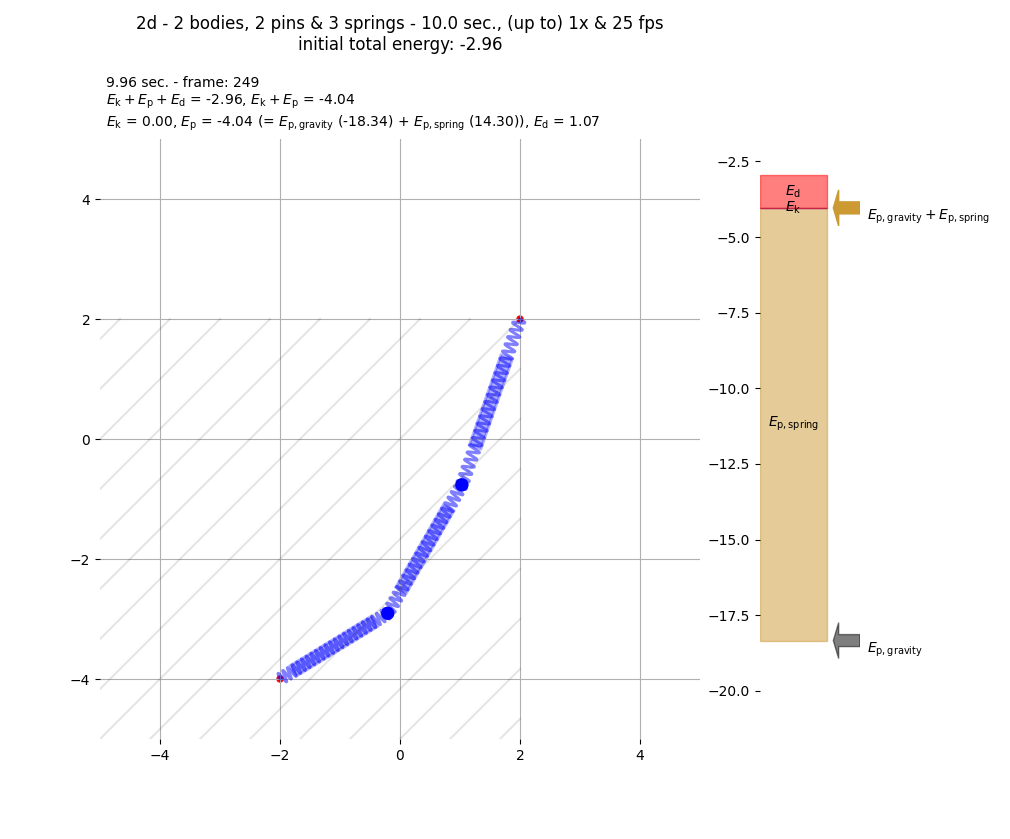
\includegraphics[trim=180 100 350 220, clip, width=.35\textwidth]{figures/2d-2-bodies-2-pins}
\end{center}
\caption{$2$ point masses and $3$ springs}
\label{fig:two-masses-and-three-springs}
\end{figure}

Note that the quantity in (\ref{eq:force:1}) equals to the sum of the forces exerted on $m_1$
and that in (\ref{eq:force:2}) equals to the sum of the forces exerted on $m_2$.
Therefore (at least for this case)
it has been shown that the configuration where the sum of all potential energies is minimized
is the same as that where the sum of the forces exerted on each mass is zero.

\subsubsection{Numerical solution}

One can solve the system of equations (\ref{eq:force:1}) and (\ref{eq:force:2})
using an iterative method such as \href{https://en.wikipedia.org/wiki/Newton%27s_method}{Netwon's method} as follows~\cite{Newton-Raphson}.
Define a function $F:\reals^6 \to \reals^6$
such that
\[
F(x) = F(x_1,x_2) = \begin{my-matrix}{c}
-\frac{\partial}{\partial x_1} f(x_1,x_2)
\\
-\frac{\partial}{\partial x_2} f(x_1,x_2)
\end{my-matrix}
\in\reals^6
\]
where $x=(x_1,x_2)\in\reals^6$
and
each term is equal to (\ref{eq:force:1}) and (\ref{eq:force:2}) respectively.
Given some initial point $x^0\in\reals^6$,
one can repeat the following procedure for $k=1,2,\ldots$
\begin{equation}
	x^{k+1} = x^k - \alpha_k DF(x^k)^{-1} F(x)
\end{equation}
where $DF:\reals^6 \to \reals^{6\times 6}$ is the Jacobian matrix of $F$
and $0<\alpha_k<1$ is step lengths for each iterate.

\subsubsection{Way easier, but approximate, solution method}

While the function $f:\reals^6 \to\reals$ in (\ref{eq:sum-of-potential-energies}) is not a convex function,
hence it is not easy to minimize (we need some definition of \emph{easiness} here!),
we can easily, but approximately, minimize the function
by letting $l_1=l_2=l_3=0$.
If $l_1=l_2=l_3=0$,
$f$ in (\ref{eq:sum-of-potential-energies})
becomes
\begin{equation}
\label{eq:sum-of-potential-energies-convex}
\tilde{f}(x_1,x_2)
= \frac{k_1}{2} \|x_1-y_1\|^2
+\frac{k_2}{2} \|x_1-x_2\|^2
+\frac{k_3}{2} \|x_2-y_2\|^2
-a^T(m_1x_1+m_2x_2),
\end{equation}
hence a convex function~\cite{BV:04},
and the partial derivatives are
\begin{equation}
\label{eq:1}
-\frac{\partial}{\partial x_1} f(x_1,x_2) = -k_1 (x_1-y_1) -k_2(x_1-x_2) + m_1 a = 0
\in\reals^3
\end{equation}
and
\begin{equation}
\label{eq:2}
-\frac{\partial}{\partial x_2} f(x_1,x_2) = -k_2 (x_2-x_1) -k_3(x_2-y_2) + m_2 a = 0
\in\reals^3.
\end{equation}

Note that the system of equations (\ref{eq:1}) and (\ref{eq:2})
is just a linear system because they are equivalent to
\begin{equation}
\label{eq:lin-system}
\begin{my-matrix}{cc}
(k_1 + k_2)I_3 & -k_2I_3
\\
-k_2 I_3 & (k_2+k_3)I_3
\end{my-matrix}
\begin{my-matrix}{c}
x_1
\\
x_2
\end{my-matrix}
=
\begin{my-matrix}{c}
m_1a
\\
m_2a
\end{my-matrix}
\end{equation}
which is nothing but a (simple) linear system
\begin{equation}
Ax = b
\end{equation}
with
\[
A=
\begin{my-matrix}{cc}
(k_1 + k_2)I_3 & -k_2I_3
\\
-k_2 I_3 & (k_2+k_3)I_3
\end{my-matrix}
\in\reals^{6\times 6},
\quad
b=
\begin{my-matrix}{c}
m_1a
\\
m_2a
\end{my-matrix}
\in\reals^6.
\]

Using a modern computer system and the numerical packages (that have been developed for decades by amazing experts based on amazing research results),
any linear system can be solved extremely fast, stably, and efficiently
\emph{even for hundreds of thousands of variables}.
Therefore one can obtain the solution for (\ref{eq:lin-system}) very easily.

Hence, we can use this solution for a surrogate for the equilibrium point
to find the lowest energy point fast and easily
for \emph{an arbitrarily complicated and large system}.

If you turn on the \verb+minimize_energy+ as below,
{\tt science} will calculate this \emph{approximate} lowest energy configuration
and will put the point masses at those points initially.

\begin{verbatim}
simulation_setting:
  minimize_energy: true
\end{verbatim}


\section{Simple harmonic motions}
\label{section:simple-harmonic-motions}

\subsection{Spring}

\subsubsection{Without frictional force}

Suppose a (point) mass $m$ is attached to a spring with spring constant $k$.
Suppose also hat $x:\preals\to\reals$ is the displacement of the mass from the natural length of the spring,
which is a function of time $t$.
The Newton's second law dictates that
\begin{equation}
\label{eq:ode:spring-harmonic-no-attenuation}
	m \ddot{x}(t)
	=
	-kx(t)
\end{equation}
where we define
\[
	\ddot{x}(t) = \frac{d}{dt^2} x(t).
\]

This is what is called an \href{https://en.wikipedia.org/wiki/Ordinary_differential_equation}{ordinary differential equation (ODE)}.
We could use some fancy techniques such as \href{https://en.wikipedia.org/wiki/Laplace_transform}{Laplace transform}~\cite{Laplace-transform}
(which has some advantages, \eg, effortlessly taking into account the initial conditions),
but we will \emph{NOT} use such methods
because we can achieve the very same thing with much easier methods as will be seen below.

Because we know the motion dictates by (\ref{eq:ode:spring-harmonic-no-attenuation}) is a harmonic motion,
we can assume it is of the form
\begin{equation}
\label{eq:harmonic-gen-sol}
	x(t) = A \cos(\omega t + \theta_0)
	= A \cos(2\pi f t + \theta_0)
\end{equation}
for some $A>0$, $\omega=2\pi f >0$, and $0\leq \theta_0 <2\pi$.
Here $\omega$ is called an \emph{angular frequency}
and $f$ just a \emph{frequency}.

Now if we plug (\ref{eq:harmonic-gen-sol}) in (\ref{eq:ode:spring-harmonic-no-attenuation}),
we have
\[
-m \omega^2 x(t) = - k x(t)
\]
which gives
\begin{equation}
\label{eq:freq-sol}
\omega = \sqrt{k/m}
\quad
\Leftrightarrow
\quad
f = \sqrt{k/m} / 2\pi
\end{equation}

We can confirm this formula by using our dynamic simulation tool, {\tt science}.
Here are some examples, which are the results of the simulation by {\tt science}.

\begin{itemize}
\item
{\tt \href{https://github.com/sungheeyun/science/blob/main/animations/1d-spring-harmonic-motion-0.5-Hz.gif}{1d-spring-harmonic-motion-0.5-Hz.gif}}
\item
{\tt \href{https://github.com/sungheeyun/science/blob/main/animations/1d-spring-harmonic-motion-1-Hz.gif}{1d-spring-harmonic-motion-1-Hz.gif}}
\item
{\tt \href{https://github.com/sungheeyun/science/blob/main/animations/1d-spring-harmonic-motion-2-Hz.gif}{1d-spring-harmonic-motion-2-Hz.gif}}
\end{itemize}

Note that the other two parameters, $A$ and $\theta_0$, are determined by the initial conditions,
that is, the initial location $x(0)$ and the initial velocity $\dot{x}(0)$.
Because we have $2$ variables and $2$ equations,
those are uniquely determined by those equations.


\subsubsection{With frictional force}
\label{subsubsection:spring-with-frictional-force}

Here we assume that the frictional force exerts on $m$,
the magnitude of which is proportional to the velocity
(and, of course, the direction is the opposite of the velocity),
as described in \S\ref{subsection:frictional-forces}.

Again the Newton's second law dictates that
\begin{equation}
\label{eq:ode:spring-harmonic-attenuation}
	m \ddot{x}(t)
	=
	-kx(t) - c \dot{x}(t)
\end{equation}
where we define
\[
	\dot{x}(t) = \frac{d}{dt} x(t).
\]

This is also an ODE and we also can use fancy methods like Laplace transform, but again we avoid using it here.
(The readers who are interested in learning how one can do this using Laplace transform
may want to refer to \S\ref{app:section:harmonic-motion-via-laplace-transform}.)
We know that the solution to (\ref{eq:ode:spring-harmonic-attenuation})
is of the form
\begin{equation}
\label{eq:harmonic-gen-sol-attenuation}
	x(t) = A e^{-at} \cos(\omega t + \theta_0)
	= A e^{-at}\cos(2\pi f t + \theta_0)
\end{equation}
for some $A>0$, $a>0$, $\omega=2\pi f >0$, and $0\leq \theta_0 <2\pi$.
Note the difference between (\ref{eq:harmonic-gen-sol}) and (\ref{eq:harmonic-gen-sol-attenuation}),
that is,
we have an attenuation term,
which exponentially reduces the magnitude of the harmonic motion.
Instead of dealing with this solution dependent of four parameters, $A$, $a$, $\omega$, and $\theta_0$,
we can (equivalently) deal with the below solution with two complex parameters, $\alpha,\beta\in\complexes$.
\begin{equation}
\label{eq:harmonic-gen-sol-complex}
x(t) = \exp(\alpha t + \beta)
\end{equation}
Note that they have the same degrees of freedom (so to speak).

Once again,
let us plug (\ref{eq:harmonic-gen-sol-complex}) in (\ref{eq:ode:spring-harmonic-attenuation})
to obtain
the quadratic equation:
\begin{equation}
\label{eq:quad}
m \alpha^2 x(t) = -k x(t) - c \alpha x(t)
\quad
\Leftrightarrow
\quad
m \alpha^2 + c \alpha + k = 0
\end{equation}

The solution of (\ref{eq:quad}) characterizes the (harmonic) attenuated motion. Using the quadratic formula,
we obtain the solution.
\[
\alpha = \frac
{-c \pm \sqrt{c^2 - 4mk}}
{2m}
\]

First, if $c > 2\sqrt{mk}$, then $\alpha$ is a real number,
hence there is no harmonic motion, but only attenuation. This is shown at
{\tt \href{https://github.com/sungheeyun/science/blob/main/animations/1d-spring-attenuation-motion.gif}{1d-spring-attenuation-motion.gif}}.

Now if $c<2 \sqrt{mk}$, we can rewrite the solution as below:
\[
\alpha =
-b
\pm
i \omega
\]
where
\begin{equation}
\label{eq:attenuation-coefficient}
b= {c}/ {2m}
\end{equation}
and
\begin{equation}
\label{eq:angular-frequency}
\omega
= {\sqrt{4mk-c^2}}/ {2m}
= \sqrt{k/m - (c/2m)^2}.
\end{equation}

If we plug this solution in (\ref{eq:harmonic-gen-sol-complex}),
we obtain
\begin{equation}
\label{eq:sol-spring-with-friction}
	x(t) =  A e^{-bt} \cos(\omega t + \theta_0)
\end{equation}
with some $A>0$ and $0\leq \theta_0 < 2\pi$,
which are determined by $\beta$ in (\ref{eq:harmonic-gen-sol-complex}),
which again are determined by the initial conditions,
\ie,
$x(0)$ and $\dot{x}(0)$.

This gives an attenuated harmonic motion,
that is,
it oscillates, but the amplitude of the oscillation reduces exponentially.
The attenuation rate is determined by $b$
and the frequency of the oscillation is determined by $\omega$ (of course).
One such example is shown at
{\tt \href{https://github.com/sungheeyun/science/blob/main/animations/1d-spring-attenuated-harmonic-motion.gif}{1d-spring-attenuated-harmonic-motion.gif}}

Note that $c=0$ (of course) gives us the same solution as in (\ref{eq:freq-sol}).

(Note that I've omitted some technical arguments here, but please trust me on that
the solutions we have derived are correct.)

\section{Dynamic system analysis, design, and verification}

From the derivations in \S\ref{section:simple-harmonic-motions},
we note several tasks we can do using those formula.

\paragraph{System analysis}

We first note that the three numbers $m$, $k$, and $c$
completely characterizes the motion,
\eg,
whether or not it will oscillates,
the attenuation rate,
and the frequency of the harmonic motion.
This means we can do the analysis of the motion
if we know exact (or even approximate) values for these parameters.

We can also do some quantitative analysis such as follows.
We know if the coefficient of friction gets large,
the mass will stop faster (\ie, earlier).
This may sound obvious,
but what the formula provides is the attenuation coefficient is exactly proportional to the coefficient of friction $c$,
\eg,
not to the square of $c$ (if you know what I mean).
I also know that if $m$ gets larger,
the mass will stops slower (\ie, later),
and the attenuation coefficient is exactly inversely proportional to $m$.
Similarly,
not only do we know that when $c$ gets smaller, the frequency gets larger,
but that exactly how much it gets larger from (\ref{eq:angular-frequency}).

\paragraph{System design}

On the other hand,
we can design a system
using the formula we have derived in \S\ref{subsubsection:spring-with-frictional-force},
\ie,
we know how we should design the system to achieve the attenuation rate or frequency we want
by deciding,
\eg,
the stiffness of the spring,
the mass,
or the coefficient of friction.

\paragraph{System verification}

Finally we can verify the motions using software such as we develop in this project {\tt science}.
Note that we can exactly design simple systems such as the one we show for the analysis here,
it is in general impossible to derive such exact closed form equations
in general cases,
\eg, where there exist hundreds of point masses, thousands of springs, and lots of diverse friction forces.
To make the situation even more complicated,
we sometimes have to model the frictional forces and spring forces, for example,
using quite advanced modeling technique, not just a simple assumption that they will be proportional to the velocity and the displacement.
The software such as {\tt science} provides a great verification tool even for such cases.

In real world, the verification is crucial for virtually every industry field.
Typical examples include
semiconductor chip design and manufacturing,
aircraft design and manufacturing,
and still other great number of mission critical tasks.

\appendix
\section{Harmonic motion via Laplace transform}
\label{app:section:harmonic-motion-via-laplace-transform}

The Laplace transform $X:\complexes\to\complexes$ of $x:\preals\to\reals$ is defined by
\begin{equation}
X(s) = \int_{0}^\infty x(t) e^{-st} dt
\end{equation}
where $x\in\complexes$.
If we take Laplace transform~\cite{Laplace-transform} on both sides of the ODE (\ref{eq:ode:spring-harmonic-attenuation}),
we have
\[
	m (s^2X(s) -s x(0) - \dot{x}(0))
	=
	-kX(x)
	-c(sX(s) - x(0) )
\]
which is equivalent to
\begin{equation}
(ms^2 + cs + k ) X(s) = smx(0) + m\dot{x}(0) + cx(0).
\end{equation}

Let $\gamma$ and $\delta$ be the two (distinct) roots of the quadratic equation,
then
\[
X(s)
=
\frac{
sx(0) + \dot{x}(0) + cx(0)/m
}{
(s-\gamma)(s-\delta)
}
=
\frac{C}{s-\gamma}
+
\frac{D}{s-\delta}
\]
%\begin{eqnarray*}
%C + D &=& x(0)
%\\
%\delta C + \gamma D  &=& -(\dot{x}(0) + cx(0)/m)
%\end{eqnarray*}
where
\begin{eqnarray*}
C &=&
\frac{
\gamma x(0) +(\dot{x}(0) + cx(0)/m)
}{
\gamma-\delta
}
\\
D &=&
-
\frac{
\delta x(0) +(\dot{x}(0) + cx(0)/m)
}{
\gamma-\delta
}
\end{eqnarray*}
hence
\[
x(t) = C e^{\gamma t} + D e^{\delta t}.
\]

In case that $c < s\sqrt{mk}$,
we have $\gamma=-b +  i \omega$ and $\delta = -b - i \omega$
where
$
b= {c}/ {2m}
$
and
$
\omega
= {\sqrt{4mk-c^2}}/ {2m}
= \sqrt{k/m - (c/2m)^2}$.
Then
\begin{eqnarray*}
C &=&
\frac{
(-b+i\omega) x(0) +(\dot{x}(0) + cx(0)/m)
}{
2i\omega
}
= \frac{x(0)}{2}
- i\frac{\dot{x}(0) + (c/m-b)x(0)}{2\omega}
=\frac{A}{2} e^{ i \theta_0}
\\
D &=&
\frac{
(b+i\omega) x(0) - (\dot{x}(0) + cx(0)/m)
}{
2i\omega
}
=
\frac{x(0)}{2}
+
i
\frac{
\dot{x}(0) + (c/m-b)x(0)
}{
2\omega
}
=\frac{A}{2} e^{- i \theta_0}
\end{eqnarray*}
for some $A>0$ and $0\leq \theta_0 < 2\pi$,
hence $D = \overline{C}$ and
\[
x(t) = C e^{\gamma t} + \overline{C e^{\gamma t}}
=  2 \Re (C e^{\gamma t} )
=  A \Re (e^{(-b+i\omega) t+i\theta_0} )
= A  e^{-bt} \cos(\omega t + \theta_0)
\]
which coincides with the solution (\ref{eq:sol-spring-with-friction}) found in \S\ref{subsubsection:spring-with-frictional-force}.



%\bibliographystyle{unsrt}
%\bibliographystyle{abbrv}
%\bibliographystyle{acm}
%\bibliographystyle{apalike}
%\bibliographystyle{alpha}
%\bibliographystyle{ieeetr}
\bibliographystyle{plain}
%\bibliographystyle{siam}
\bibliography{../../FrequentlyUsed/latex/mybib}

\end{document}
